%%%%%%%%%%%%%%%%%%%%%%%%%%%%%%%%%%%%%%%%%%%%%%%%%%%%%%%%%%%%
%%  This Beamer template was created by Cameron Bracken.
%%  Anyone can freely use or modify it for any purpose
%%  without attribution.
%%
%%  Last Modified: January 9, 2009
%%

%\documentclass[xcolor=x11names,compress,8pt]{beamer}
\documentclass[xcolor=x11names,compress,8pt,
%handout
]{beamer}

%%% langue
\usepackage[francais]{babel}

\usepackage[T1]{fontenc}
\usepackage[utf8]{inputenc}

\def\mytoday{%\number\day\space
 \ifcase\month\or
 January\or February\or March\or April\or May\or June\or
July\or August\or September\or October\or November\or December\fi
 \space\number\year}


%%% mathématiques
\usepackage{amsmath,amsfonts,amssymb,newlfont,latexsym}

 \def\leq{\leqslant}
 \def\geq{\geqslant}
 
 \def\real{\mathbb{R}}
 \def\Prob{\mathbb{P}}
 
 \def\integer{\mathbb{N}}
 \def\relative{\mathbb{Z}}
 \def\Esp{\mathbb{E}}

%%%%% hyperliens
\usepackage{hyperref,url}
\hypersetup{
dvips,
backref=true, %permet d'ajouter des liens dans...
pagebackref=true,%...les bibliographies
hyperindex=true, %ajoute des liens dans les index.
colorlinks=true, %colorise les liens
breaklinks=true, %permet le retour à la ligne dans les liens trop longs
urlcolor= blue, %couleur des hyperliens
linkcolor= blue, %couleur des liens internes
bookmarks=true, %créé des signets pour Acrobat
bookmarksopen=true} 

%% General document %%%%%%%%%%%%%%%%%%%%%%%%%%%%%%%%%%
\usepackage{graphicx}

\graphicspath{{logos/}{images/}{figures/}{photos/}}

\usepackage{figlatex}%

%\usepackage{tikz}
%\usepackage{pgfplots}

%\usetikzlibrary{decorations.fractals}
%%%%%%%%%%%%%%%%%%%%%%%%%%%%%%%%%%%%%%%%%%%%%%%%%%%%%%


%% Beamer Layout %%%%%%%%%%%%%%%%%%%%%%%%%%%%%%%%%%
\useoutertheme[subsection=false,shadow]{miniframes}
\useinnertheme{default}
%\usefonttheme{serif}
\usepackage{palatino}

\usepackage{xcolor}
\usepackage{colortbl}
\usepackage{soul}
\sethlcolor{Green44}
\definecolor{gris05}{gray}{0.95}

\setbeamerfont{title like}{shape=\scshape}
\setbeamerfont{frametitle}{shape=\scshape}

\setbeamercolor*{lower separation line head}{bg=DeepSkyBlue4} 
\setbeamercolor*{normal text}{fg=black,bg=white} 
\setbeamercolor*{alerted text}{fg=IndianRed4} 
\setbeamercolor*{example text}{fg=black} 
\setbeamercolor*{structure}{fg=black} 

\setbeamercolor*{palette tertiary}{fg=black,bg=black!10} 
\setbeamercolor*{palette quaternary}{fg=black,bg=black!10} 

\renewcommand{\(}{\begin{columns}}
\renewcommand{\)}{\end{columns}}
\newcommand{\<}[1]{\begin{column}{#1}}
\renewcommand{\>}{\end{column}}
%%%%%%%%%%%%%%%%%%%%%%%%%%%%%%%%%%%%%%%%%%%%%%%%%%
\usefonttheme{progressbar}
\useoutertheme{progressbar}
\useinnertheme{progressbar}


\setbeamertemplate{itemize item}[triangle]  
\setbeamertemplate{enumerate item}[diamond] 

\setbeamertemplate{navigation symbols}{}

%\beamertemplatetransparentcovereddynamic

% \setbeamercovered{transparent}

\pgfdeclareimage[height=0.5cm]{university-logo}{logos/logoUGA.jpg}
  
\logo{\pgfuseimage{university-logo}}

\title[Data Characterization] % (optional, use only with long paper titles)
{Sample Quality}
\subtitle{descriptive analysis of data}

\author% (optional, use only with lots of authors)
{		
Lucas Mello Schnorr, Jean-Marc Vincent
}
% - Give the names in the same order as the appear in the paper.
% - Use the \inst{?} command only if the authors have different
%   affiliation.

\institute[LICIA] % (optional, but mostly needed)
{%
{\large INF/UFRGS\\
Porto Alegre, Brazil – \mytoday}
}
% - Use the \inst command only if there are several affiliations.
% - Keep it simple, no one is interested in your street address.

\date[Porto Alegre 2018] % (optional, should be abbreviation of conference name)
{

\includegraphics[width=2cm]{logos/ufrgs2.png}\hfill

\includegraphics[width=2cm]{logos/licia-small.png}\hfill

\includegraphics[width=2cm]{logos/uga.png}
}



% \AtBeginSection[]
%{
%  \begin{frame}<beamer>
%    \frametitle{}
%    \tableofcontents[currentsection]
%  \end{frame}
%}

\begin{document}

\begin{frame}
\titlepage
\end{frame}
%%%%%%%%%%%%%%%%%%%%%%%%%%%%%%%%%%%%%%%%%%%%%
\section[{\scshape Global Control}]{{\scshape Global Control}}

\begin{frame}{Control of experiments (1)}
\begin{center}
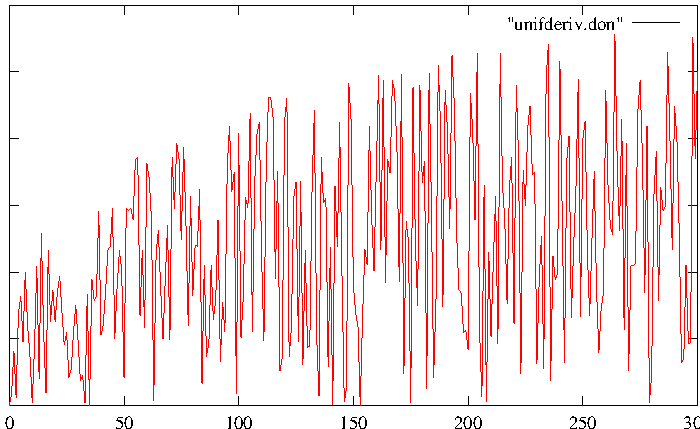
\includegraphics[width=5.5cm]{CE-unifderiv.pdf}
\end{center}
\pause
\begin{block}{Tendency analysis}
\alert{\bf non homogeneous experiment}

$\Rightarrow$ model the evolution of experiment

estimate and compensate tendency

\textcolor{blue}{\bf explain why}
\end{block}
\end{frame}
\begin{frame}{Control of experiments (2)}
\begin{center}
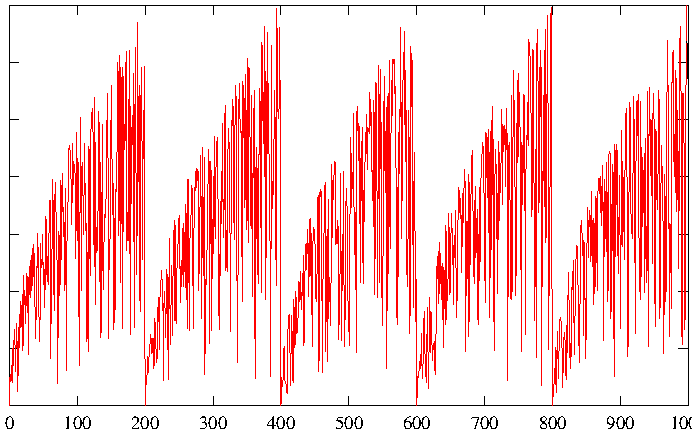
\includegraphics[width=5.5cm]{CE-periode.pdf}
\end{center}
\pause
\begin{block}{Periodicity analysis}
\alert{\bf periodic evolution of the experimental environment ?}

$\Rightarrow$ model the evolution of experiment

Fourier analysis of the sample

Integration on time (sliding window analysis) Danger : size of the window

Wavelet analysis

\textcolor{blue}{\bf explain why}
\end{block}
\end{frame}
\begin{frame}{Control of experiments (3)}
\begin{center}
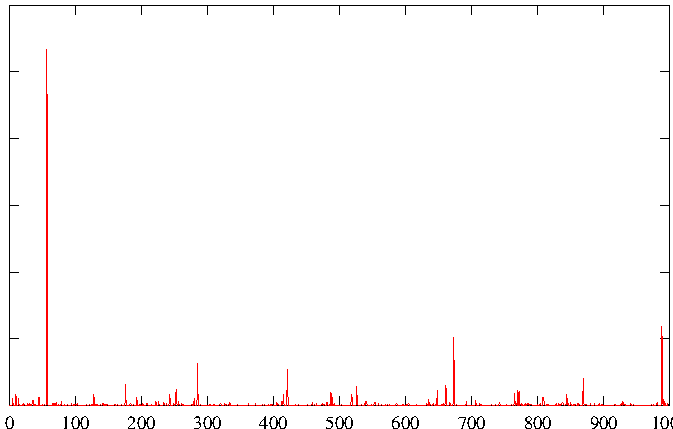
\includegraphics[width=5.5cm]{CE-cauchy1.pdf}
\end{center}
\pause
\begin{block}{Non significant values}
\alert{\bf  extraordinary behaviour of experimental environment}

rare events with different orders of magnitude

$\Rightarrow$ threshold by value \\
Danger : choice of the threshold : indicate the rejection rate

$\Rightarrow$ threshold by quantile \\
Danger : choice of the percentage : indicate the rejection value

\textcolor{blue}{\bf explain why}
\end{block}
\end{frame}

\begin{frame}{Control of experiments (4)}
Threshold value : 10
\begin{center}
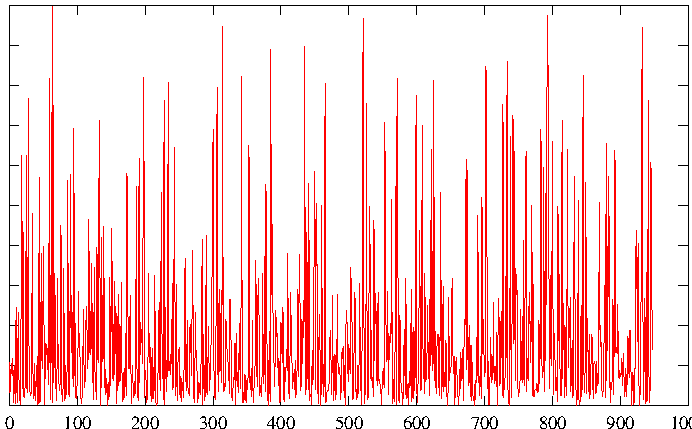
\includegraphics[width=5cm]{CE-cauchy-seuil10.pdf}
\end{center}
Threshold percentage  : 1\%
\begin{center}
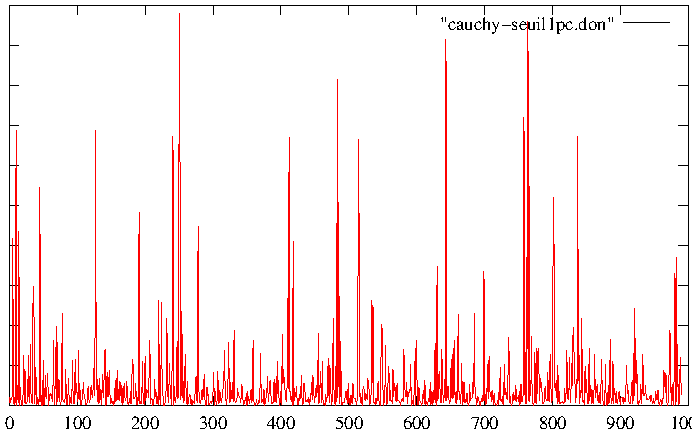
\includegraphics[width=5cm]{CE-cauchy-seuil1pc.pdf}
\end{center}

\end{frame}
\begin{frame}{Control of experiments (5)}
\begin{center}
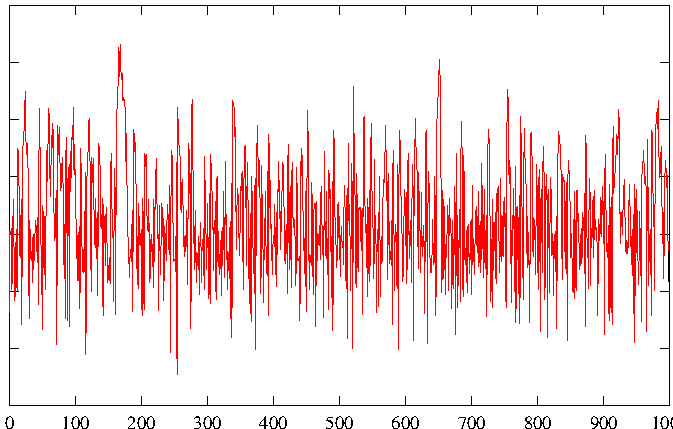
\includegraphics[width=5.5cm]{CE-deptempo.pdf}
\end{center}
\pause
\begin{block}{}
\alert{\bf  looks like correct experiments}

Statistically independent

Statistically homogeneous
\end{block}
\end{frame}

\begin{frame}{Control of experiments (5bis)}
Zooming
\begin{center}
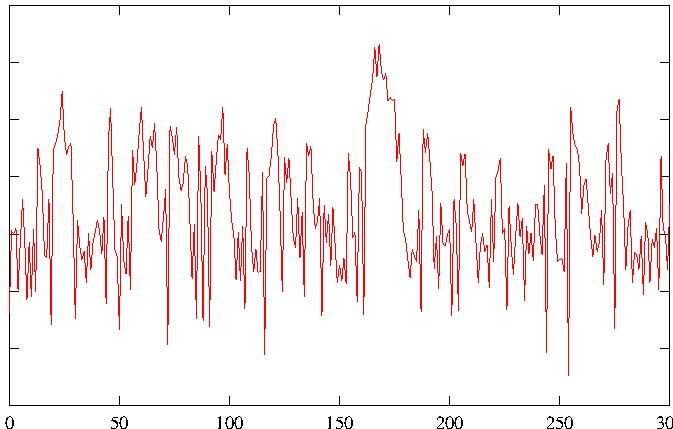
\includegraphics[width=5.5cm]{CE-deptempo-zoom.pdf}
\end{center}
\pause
\begin{block}{Autocorrelation}
Danger time correlation among samples

\alert{\bf  experiments impact on experiments}

$\Rightarrow$ stationarity analysis

autocorrelation estimation (ARMA)
\end{block}
\end{frame}
\section[{\scshape Sample Analysis}]{{\scshape Sample Analysis}}

\section{Analysis of Experiments}
\begin{frame}{Experimental results}
\begin{itemize}
\item Deterministic (controlled error non significant (white noise))
\item Statistic (the system is non deterministic)
\end{itemize}
\begin{block}{Sample analysis}
\begin{itemize}
\item Identification of the response set
\item Structure of the response set (measure)
\end{itemize}

\end{block}
\end{frame}

\begin{frame}{Distribution  analysis}
Summarize data in a {\bf histogram}
\begin{center}
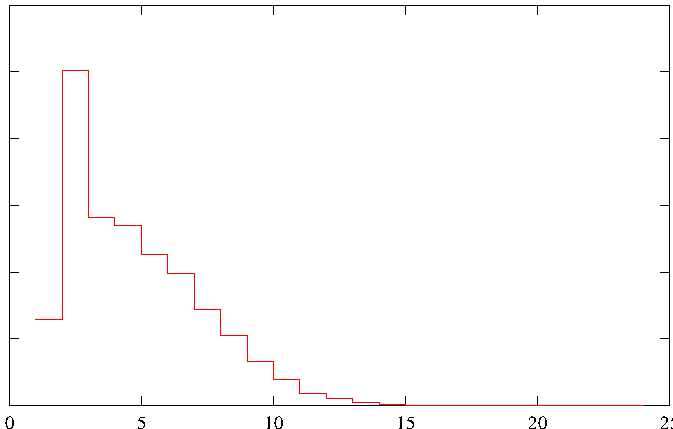
\includegraphics[width=4.6cm]{histogramme.pdf}
\end{center}
\begin{block}{Shape analysis}
\begin{itemize}
\item unimodal / multimodal
\item variability
\item symmetric / dissymmetric (skewness)
\item flatness (kurtosis)
\end{itemize}
\alert{\bf $\Longrightarrow$ Central tendency analysis} 

\alert{\bf $\Longrightarrow$ Variability analysis around the central tendency} 

\end{block}
\end{frame}
\section[{\scshape Central Tendency}]{{\scshape Central Tendency}}
\begin{frame}{Mode value}
{\bf histogram}
\begin{center}
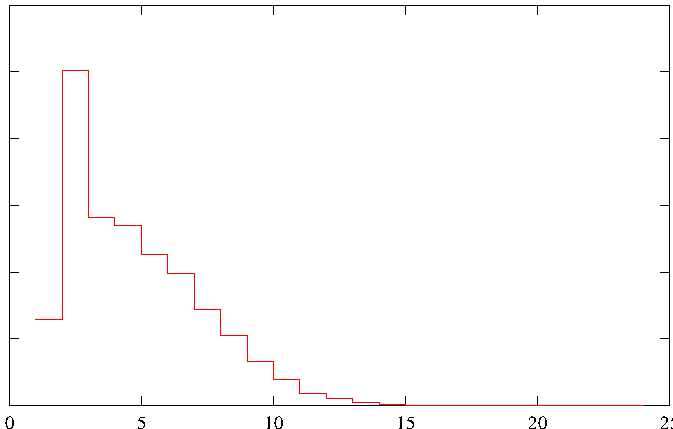
\includegraphics[width=4.6cm]{histogramme.pdf}
\end{center}
\begin{block}{Mode}
\begin{itemize}
\item  {\textcolor{Green4}{\bf Categorical data}}
\item Most frequent value
\item highly unstable value
\item for continuous value distribution depends on the histogram step
\item interpretation depends on the flatness of the histogram
\end{itemize}
\alert{\bf $\Longrightarrow$ Use it carefully} 

\alert{\bf $\Longrightarrow$ Predictor function} 

\end{block}
\end{frame}
\begin{frame}{Median value}
{\bf histogram}
\begin{center}
%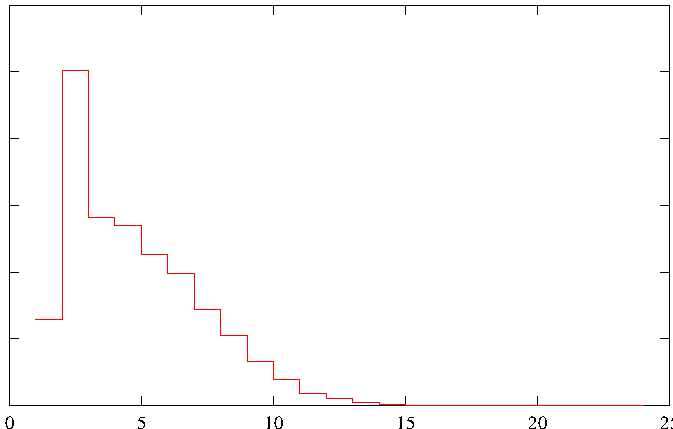
\includegraphics[width=4.6cm]{histogramme.pdf}
\end{center}
\begin{block}{Median}
\begin{itemize}
\item {\textcolor{Green4}{\bf Ordered data}}
\item Split the sample in two equal parts 
\[
\sum_{i\leq Median}f_i \leq \frac 1 2 \leq \sum_{i\leq Median+1}f_i .\]
\item more stable value
\item does not depends on the histogram step 
\item difficult to combine (two samples)
\end{itemize}


\alert{\bf $\Longrightarrow$ Randomized algorithms} 

\end{block}
\end{frame}
\begin{frame}{Mean value}
{\bf histogram}
\begin{center}
%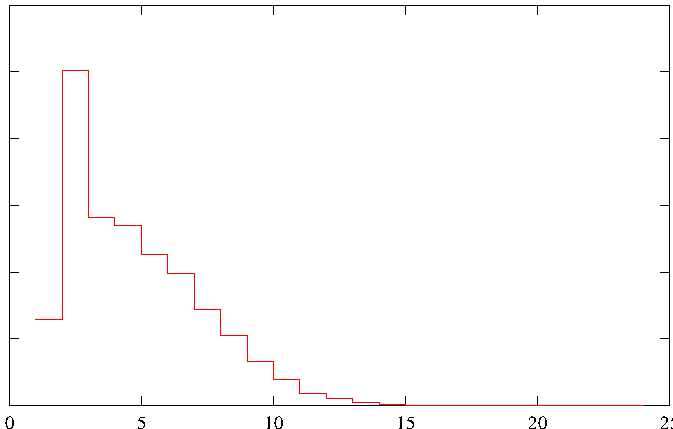
\includegraphics[width=4.6cm]{histogramme.pdf}
\end{center}
\begin{block}{Mean}
\begin{itemize}
\item {\textcolor{Green4}{\bf Vector space}}
\item Average of values 
\[
Mean = \frac 1 {Sample\_Size}\sum x_i = \sum_{x}x.f_x .\]
\item stable value 
\item does not depends on the histogram step 
\item easy to combine (two samples $\Rightarrow$ weighted mean)
\end{itemize}


\alert{\bf $\Longrightarrow$ Additive problems (cost, durations, length,...)} 

\end{block}
\end{frame}
\begin{frame}{Central tendency}
{\bf histogram}
\begin{center}
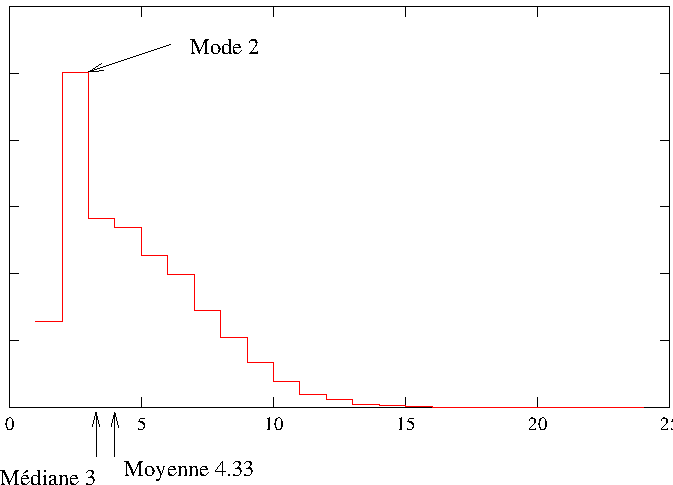
\includegraphics[width=4.6cm]{histogramme2.pdf}
\end{center}
\begin{block}{Complementarity}
\begin{itemize}
\item Valid if the sample is "Well-formed"
\item {\textcolor{Green4}{\bf Semantic of the observation}}
\item Goal of analysis 
\end{itemize}

\alert{\bf $\Longrightarrow$ Additive problems (cost, durations, length,...)} 

\end{block}
\end{frame}
\begin{frame}{Central tendency (2)}
\begin{block}{Summary of Means}
\begin{itemize}
\item Avoid means if possible\\
Loses information
\item  \textcolor{blue}{Arithmetic mean}\\
 When sum of raw values has physical meaning\\
Use for summarizing times (not rates)
\item \textcolor{blue}{Harmonic mean}\\
Use for summarizing rates (not times)
\item \textcolor{blue}{Geometric mean}\\
 Not useful when time is best measure of perf\\
 Useful when multiplicative effects are in play
\end{itemize}
\end{block}
\end{frame}
\section[{\scshape Variability}]{{\scshape Variability}}

\begin{frame}{Variability}
\begin{block}{Categorical data (finite set)}
$f_i$ : empirical frequency of element $i$

Empirical entropy
\[
H(f)=\sum_i f_i \log f_i.\]
Measure the empirical distance with the uniform distribution
\begin{itemize}
\item $H(f)\geq 0$
\item $H(f)=0$ iff the observations are reduced to a unique value
\item $H(f)$ is maximal for the uniform distribution
\end{itemize} 
\end{block}
\end{frame}
\begin{frame}{Variability (2)}
\begin{block}{Ordered data }

Quantiles : quartiles, deciles, etc

Sort the sample : 
\[
(x_1,x_2,\cdots ,x_n)\longrightarrow  (x_{(1)},x_{(2)},\cdots ,x_{(n)});\]
\[
Q_1=x_{(n/4)};\; Q_2=x_{(n/2)}=Median;\; Q_3=x_{(3n/4)}.\]

For deciles
\[
d_i = argmax_i \{\sum_{j\leq i}f_j \leq \frac i {10}\}.\]
Utilization as quantile/quantile plots to compare distributions
\end{block}
\end{frame}
\begin{frame}{Variability (3)}
\begin{block}{ Vectorial data }

Quadratic error for the mean 
\[
Var(X)=\frac 1 n \sum_1^n (x_i-\bar{x}_n)^2.\]
{\bf Properties:}
\begin{eqnarray*}
Var(X) & \geq & 0;\\
Var(X)&=&\overline{x^2}-(\bar{x})^2, \;\;\mbox{where} \;\;\overline{x^2}=\frac 1 n \sum_{i=1}^n x_i^2.\;\\
Var(X+cste)&=&Var(X);\\
Var(\lambda X)&=&\lambda^2 Var(X).
\end{eqnarray*}

\end{block}
\end{frame}

\end{document}

